\documentclass[border=4pt]{standalone}
\usepackage{amsmath,amssymb,tikz}\usetikzlibrary{arrows.meta}
\definecolor{figB}{RGB}{31,90,166}\definecolor{figR}{RGB}{176,48,48}\definecolor{figG}{RGB}{46,125,50}\definecolor{figO}{RGB}{214,120,20}
\begin{document}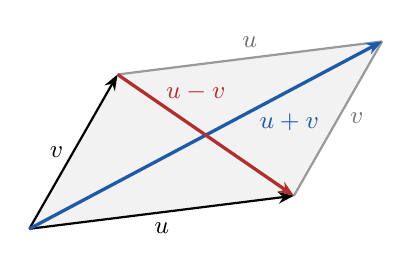
\begin{tikzpicture}[scale=1.4,>={Stealth[length=2mm]}]
\coordinate (O) at (0,0); \coordinate (U) at (2.4,0.3); \coordinate (V) at (0.8,1.4); \coordinate (S) at (3.2,1.7);
\fill[black!5] (O)--(U)--(S)--(V)--cycle;
\draw[thick,black!40] (U)--(S) node[midway,right,font=\small,black!55,inner sep=4pt]{$v$};
\draw[thick,black!40] (V)--(S) node[midway,above,font=\small,black!55]{$u$};
\draw[->,thick] (O)--(U) node[midway,below,font=\small]{$u$};
\draw[->,thick] (O)--(V) node[midway,left,font=\small]{$v$};
\draw[->,very thick,figB] (O)--(S) node[pos=0.64,below right,font=\small,inner sep=1pt]{$u+v$};
\draw[->,very thick,figR] (V)--(U) node[pos=0.25,above right,font=\small,inner sep=1pt]{$u-v$};
\end{tikzpicture}\end{document}
